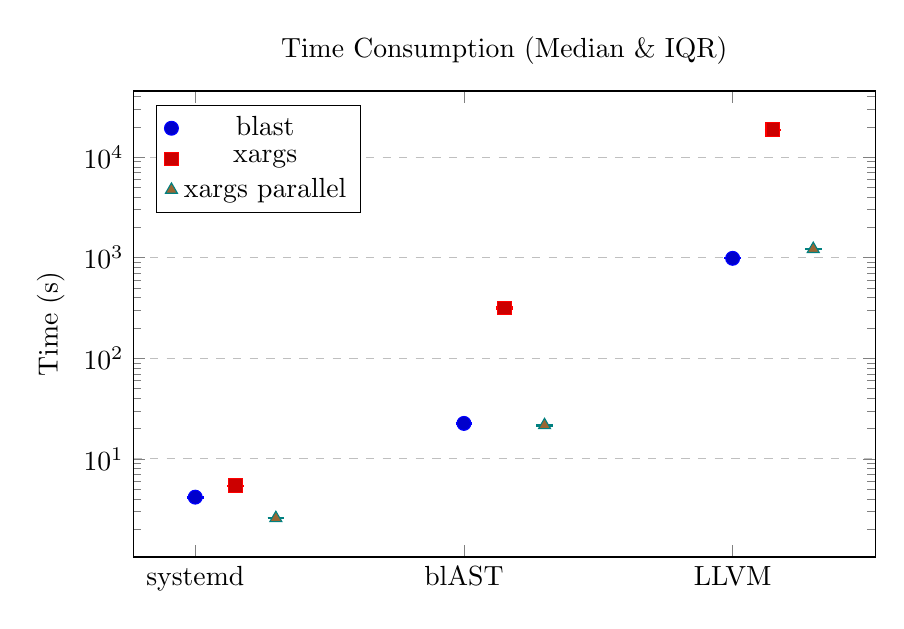
\begin{tikzpicture}
\begin{axis}[
    title={Time Consumption (Median \& IQR)},
    symbolic x coords={systemd, blAST, LLVM},
    xtick=data,
    ymode=log, % Log scale due to 4 orders of magnitude difference
    ylabel={Time (s)},
    ymajorgrids=true,
    grid style=dashed,
    legend pos=north west,
    width=11cm, height=7.5cm,
    only marks, mark size=2.5pt,
    error bars/y dir=both, error bars/y explicit,
    error bars/error bar style={line width=0.8pt},
    error bars/error mark options={rotate=90, mark size=3pt, line width=0.8pt}
]
\addplot+[color=blue, mark=*, x filter/.code={\pgfmathparse{\pgfmathresult-0.15}}] coordinates {
    (systemd, 4.17) +- (0.04, 0.04) % Q1=4.13, Q3=4.21
    (blAST, 22.55) +- (0.04, 0.13) % Q1=22.51, Q3=22.68
    (LLVM, 986.17) +- (4.01, 0.91) % Q1=982.16, Q3=987.08
};
\addlegendentry{blast}

\addplot+[color=red, mark=square*] coordinates {
    (systemd, 5.42) +- (0.01, 0.01) % Q1=5.40, Q3=5.43
    (blAST, 316.61) +- (2.25, 3.98) % Q1=314.37, Q3=320.59
    (LLVM, 18684.44) +- (3.64, 9.82) % Q1=18680.80, Q3=18694.26
};
\addlegendentry{xargs}

\addplot+[color=teal, mark=triangle*, x filter/.code={\pgfmathparse{\pgfmathresult+0.15}}] coordinates {
    (systemd, 2.58) +- (0.01, 0.00) % Q1=2.57, Q3=2.58
    (blAST, 21.65) +- (0.10, 0.19) % Q1=21.55, Q3=21.84
    (LLVM, 1220.20) +- (2.20, 6.73) % Q1=1218.00, Q3=1226.92
};
\addlegendentry{xargs parallel}

\end{axis}
\end{tikzpicture}

\vspace{1cm}

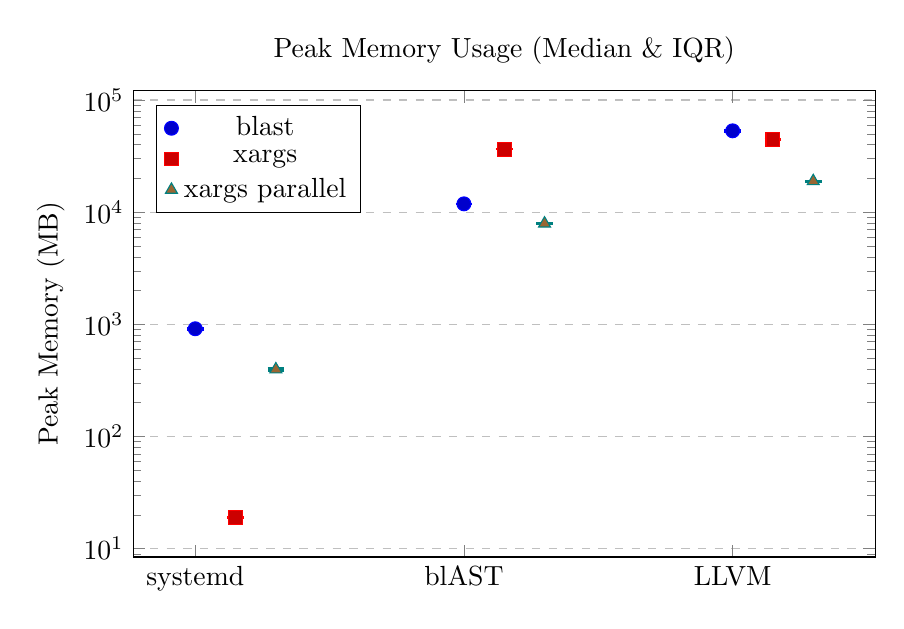
\begin{tikzpicture}
\begin{axis}[
    title={Peak Memory Usage (Median \& IQR)},
    symbolic x coords={systemd, blAST, LLVM},
    xtick=data,
    ymode=log, % Log scale due to 4 orders of magnitude difference
    ylabel={Peak Memory (MB)},
    ymajorgrids=true,
    grid style=dashed,
    legend pos=north west,
    width=11cm, height=7.5cm,
    only marks, mark size=2.5pt,
    error bars/y dir=both, error bars/y explicit,
    error bars/error bar style={line width=0.8pt},
    error bars/error mark options={rotate=90, mark size=3pt, line width=0.8pt}
]
\addplot+[color=blue, mark=*, x filter/.code={\pgfmathparse{\pgfmathresult-0.15}}] coordinates {
    (systemd, 913.44) +- (5.31, 14.21) % Q1=908.13, Q3=927.65
    (blAST, 11867.08) +- (50.63, 21.03) % Q1=11816.44, Q3=11888.11
    (LLVM, 53158.77) +- (1893.08, 1140.05) % Q1=51265.69, Q3=54298.82
};
\addlegendentry{blast}

\addplot+[color=red, mark=square*] coordinates {
    (systemd, 18.92) +- (0.61, 0.20) % Q1=18.31, Q3=19.13
    (blAST, 36376.06) +- (0.58, 0.09) % Q1=36375.48, Q3=36376.15
    (LLVM, 44630.49) +- (99.95, 241.21) % Q1=44530.55, Q3=44871.70
};
\addlegendentry{xargs}

\addplot+[color=teal, mark=triangle*, x filter/.code={\pgfmathparse{\pgfmathresult+0.15}}] coordinates {
    (systemd, 396.69) +- (10.31, 9.39) % Q1=386.39, Q3=406.08
    (blAST, 7917.75) +- (51.04, 51.15) % Q1=7866.70, Q3=7968.89
    (LLVM, 18907.41) +- (80.35, 195.90) % Q1=18827.06, Q3=19103.31
};
\addlegendentry{xargs parallel}

\end{axis}
\end{tikzpicture}
